%!TEX root = ../thesis.tex
\chapter{Background}
\label{ch:background}

\section{Hexapod Robots}
Hexapods are a type of robot featuring 6 legs, inspired by the locomotion of insects and arachnids.
Over millions of years of evolution these organisms developed efficient strategies to navigate challenging terrain, making them a rich source of inspiration for robotics.
By emulating the biomechanics and behavior of insects, researchers and engineers aim to create versatile and robust robotic systems capable of navigating challenging terrain.

Most commonly, each leg of a hexapod typically consists of 3 segments named coxa, femur and tibia, equivalent to their biological counterparts.
The individual segments are connected by 3 2-DoF(degrees of freedom) joints, each actuated by an electric servo motor.
The first joint, hereafter named \textalpha-joint, connects the coxa to the thorax(body) and moves in parallel to the ground, thus being responsible for the longitudinal placement of each leg.
Coxa and femur are connected by the \textbeta-joint, while the femur and tibia are connected by the \textgamma-joint. 
These joints move orthogonal to the movement plane of the \textalpha-joint. Together, they are responsible for the lateral positioning of each leg.




\todo{Add image of hexapod(and maybe of insect)}
\todo{CITATIONS}

\section{MATLAB}
\hiddensubsection{Simulink}
\textit{Simulink\textsuperscript{\textregistered}} is a \textit{MATLAB\textsuperscript{\textregistered}}-based graphical block-diagramming tool developed by the company \textit{MathWorks\textsuperscript{\textregistered}} .
It is a widely used tool which plays a crucial role in various engineering and research disciplines.
It provides the user with a versatile platform to design, simulate and analyze complex dynamic systems.

Simulink offers an expansive library of predefined blocks that represent different components and behaviors.
The user connects these blocks with so called signal lines to transport data between them.
Blocks transform the data provided by the inputs and output the transformed data to other blocks connected downstream.
Their behavior can be discrete, like a switch which activates when a signal is high, or represent continuous functions such as integrals.

An arrangement of blocks can be encapsulated into a subsystem, thus creating different levels of abstraction.
To enable easy reuse, subsystems can be placed in custom libraries.
If a library object gets updated, each linked copy of this subsystem receives the update as well, preventing the user from having to edit each copy themselves.
At any step in the development process, a model can be simulated and 

\hiddensubsection{Simscape}
\textit{Simscape\textsuperscript{\texttrademark}} is a block library developed by \textit{MathWorks\textsuperscript{\textregistered}} with which it is possible to model physical system within the Simulink environment.
It is capable of modeling and simulating systems such as electric circuits, hydraulics or classical mechanics all within a unified simulation environment.
The Simscape libraries offer a large variety of predefined components like resistors, capacitors, springs, dampers and more.
For this thesis, the mechanical components are of the most interest, especially rigid bodies, transforms and joints.
A model is build up using rigid bodies which get connected to coordinate frames.
These coordinate frames then get attached to each other using rigid transforms or joints.
Joints can allow different degrees of freedom between two frames, depending on what constraints should be imposed on the system.
Two frames connected with a joint are named base and follower frame.
When the joint is actuated, the follower frame moves relative to the base frame\parencite{thilderkvist2015motion}.

If the user requires a component which is not yet represented by any block in the libraries, Simscape also offers a MATLAB based language to enable text-based development of custom components.
\todo{Weiter ausführen; mehr Details, z.B. über Gelenke(Sensorik, Aktuation, etc.)}
\todo{CITATIONS}

\section{Inverse Kinematics}
Inverse Kinematics(IK) is a term predominately used in robotics and computer graphics.
It describes the process of calculating the joint angles required to place the end of a kinematic chain, such as a robotic manipulator, at a given position and orientation.
There are two distinct methods how to calculate these angles, analytical and numerical.

Analytical solvers are based on trigonometric equations derived from the geometric and kinematic parameters of the manipulator arm, such as the link length, joint type and joint limits.
They provide exact solutions to the problem and can be significantly faster than iterative approximation methods.
Although very efficient and precise, the analytical approach is generally only feasible for kinematic chains with a small number of DoF.
If for the kinematic chain the number of DoF is greater than that of the end-effector, then there exist infinite solutions for a given pose.
These kinds of systems potentially lack closed-form expressions for a solution, which makes deriving analytical solutions infeasible if not impossible.


Numerical solvers use iterate approaches to approximate the joint angles and converge towards a solution over several iterations of the algorithm.
At the start of the process this type of solver begins with an initial guess that can be based on the manipulators geometry, joint limits or previously obtained solutions.
Using the estimated joint angles, the position of the end-effector is calculated(forward kinematics) and the error between the desired pose and the currently obtained pose is determined.
Based on this error, the joint angles are adjusted with the goal to reduce the error and bringing the end-effector closer to the desired pose.
This process is repeated until the error meets the predefined tolerances.
The joint angles calculated during the final iteration are then considered a solution to the problem.
Although the basic principle of error-minimization is always present in the algorithm, the exact process of minimization is much more complex than described here and there exist numerous different techniques on how to achieve this goal.
Numerical solvers can be applied to a wide variety of inverse kinematics problems and are not limited by the number of DoF like analytical solvers.
Due to their iterative nature numerical solvers are generally more computationally expensive, given the same problem, than their analytical counterparts.

Both inverse kinematics methods are used extensively in industry and research, depending on the specific project and its requirements.
\todo{CITATIONS}




\section{PID Controller}
A \textbf{P}roportional-\textbf{I}ntegral-\textbf{D}erivative(PID) controller is a widely used feedback control system.
As such a feedback control system it aims to regulate a control variable to a desired setpoint by adjusting its output according to the currently measured process variable.
It uses three terms, proportional, integral and derivative, to compute the controlled output  based on the error between the setpoint and current process variable.
For a digital PID controller, the process of error calculation and control variable adjustment is done at a discrete fixed rate, which is also referred to as a timestep.
There also exist versions of this controller constructed using analog electronics which generate a continuous control signal, but we will focus on the digital controller here.

\todo{Insert graphic of pid controller}
At each timestep the controller first calculates the error between its setpoint and the currently measured process variable: 
\[
	Error(t) = setpoint - \textit{process variable}(t)
.\]
After the error is determined, controller continues with the propotional, integral and derivative term.

The proportional term $P(t)$ is calculated by multiplying the error by a constant factor, the so called proportional gain $K_p$.
This term contributes to the control output, as its name suggests, proportional to the magnitude of the error.
$P(t)$ is given by:
\[
	P(t) = K_p \cdot Error(t)
.\]
The integral term $I(t)$takes into account the sum of past errors to address any long term bias/ constant error contained inside of the controlled system.
It is able to eliminate long-term errors that can not be accounted for by $P(t)$.
The term is calculated by integrating the error over time and multiplying it with the integral gain $K_i$.
$I(t)$ is given by:
\[
	I(t) = K_i \cdot \int_{0}^{t} Error(\tau) \,d\tau
.\]
The derivative term $D(t)$ anticipates the errors future behavior by determining its rate of change.
It prevents the controller from overshooting and oscillating by dampening the control response.
$D(t)$ is calculated by taking the errors rate of change and multiplying it with the constant derivative gain $K_d$.
It is given by:
\[
	D(t) = K_d \cdot \frac{\partial}{\partial t}(Error(t))
.\]
The final output of the controller is the given by the sum of all three terms:
\[
	\textit{Control Output(t)} = P(t) + I(t) + D(t)
.\]
The calculated control output is the fed into the controlled system or process.
In most cases this control output corresponds to real world variable such as the speed of a motor, the liquid-level inside a tank or the temperature of an element.
The performance of a PID controller greatly depends on the values of its parameters $K_p$, $K_i$ and $K_d$.
To achieve desired results like fast response times and minimal overshooting or oscillations, these parameters have to be carefully tuned. 
To conclude, a PID controller continuously repeats the process of error calculation and adjustment, thus forming a closed-loop system which aims to minimize the error and approach the setpoint as close as possible.


\todo{CITATIONS}


\section{Reinforcement Learning}

\parencite{weng2018bandit}

\begin{figure}
	\centerline{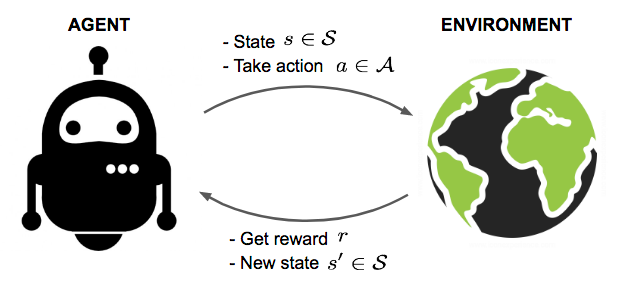
\includegraphics[scale=0.55]{rl_illustration}}
	\caption{The basic concept of Reinforcement Learning. (\cite{weng2018bandit} Fig. 1)}
	\label{RL Illustration}
\end{figure}

Model-Free vs. Model ?


Discrete vs. Continuous action space in RL learning:
A discrete action space is used when the number of actions that can be taken is limited and known in advance. An example of such an environment would be a game of chess; for each move there are only a finite amount of moves possible.
Continuous action spaces are used, when the number of actions is not known in advance and possibly infinite, such as the movement possibilities of a robotic arm.
Because we have multiple robotic 'arms' in this project, a continuous action space is favorable.

Agents applicable for continuous action spaces: 
- DDPG: Deep Deterministic Policy Gradient
- TD3: Twin-Delayed Deep Deterministic Policy Gradient (more complex improvement to DDPG)
- PPO: Proximal Policy Optimization (more stable updates, but longer training)
- SAC: Soft Actor-Critic (more complex improvement of DDPG generating stochastic policies)
- TRPO: Trust Region Policy Optimization(more complex version of PPO, more robust for deterministic environments with fewer iterations)


\todo{Use image for explanation}

\section{Swing-Stance Cycle}
\todo{add image of swing-stance cycle(Paper Schilling)}
